\section{Обзор предметной области}
\label{sec:domain}

Тайм-менеджмент – это совокупность знаний, имеющих большое не только экономическое значение, но и личное. Суть экономического значения состоит в том,
что за счет рационального использования времени возможно значительное повышение производительности труда и человека отдельно, и в целом всего
коллектива. А суть личного значения состоит в том, что оно позволяет человеку обрести достаточное количество свободного времени, благодаря которому он будет
ощущать себя более свободным, появится возможность уделять больше внимания своему здоровью, отдыху и личной жизни.

Учет времени подразумевает использование ежедневников, планнеров, составление списков дел, но не ограничивается ими. Под системой мы понимаем целостную структуру взаимосвязанных деталей, где всё вышеперечисленное является лишь элементом. В целом же система управления временем – это специальная методика, зачастую с собственным инструментарием, а также рекомендациями и советами по эффективной организации своей деятельности. Её задача – не просто напомнить о каком-либо занятии или встрече, распланировать день (месяц, год), но и показать, как это сделать эффективно, чтобы не только завершить работу в срок, но и достичь большего. В классическом понимании системы учета времени и заложена суть: она помогает человеку и планировать занятость, и гибко управлять временем, затрачиваемым на разные нужды.

Сегодня существует около десятка наиболее известных систем управления временем и множество вариаций, основанных на личном опыте их применения. На форумах и в блогах можно найти достаточное количество примеров собственных систем, где авторы объединяют элементы нескольких методик, привнося новшества, или трактуя их под свою сферу занятости. В этом, в частности, заключается одна из главных полезностей: возможность «настроить» план «под себя», изменить, полностью отбросить или позаимствовать из других техник отдельные инструкции и детали. Благодаря этому, системы управления временем может применять каждый: инженер и журналист, офисный сотрудник и фрилансер, тот, кто распределяет рабочее время и тот, кто планирует отдых. Каждая из них имеет свои преимущества, поэтому рассмотрим несколько наиболее известных.


\subsection{Пирамида Франклина}

\label{page:domain:piramida_franklina}
\begin{figure}
\centering
  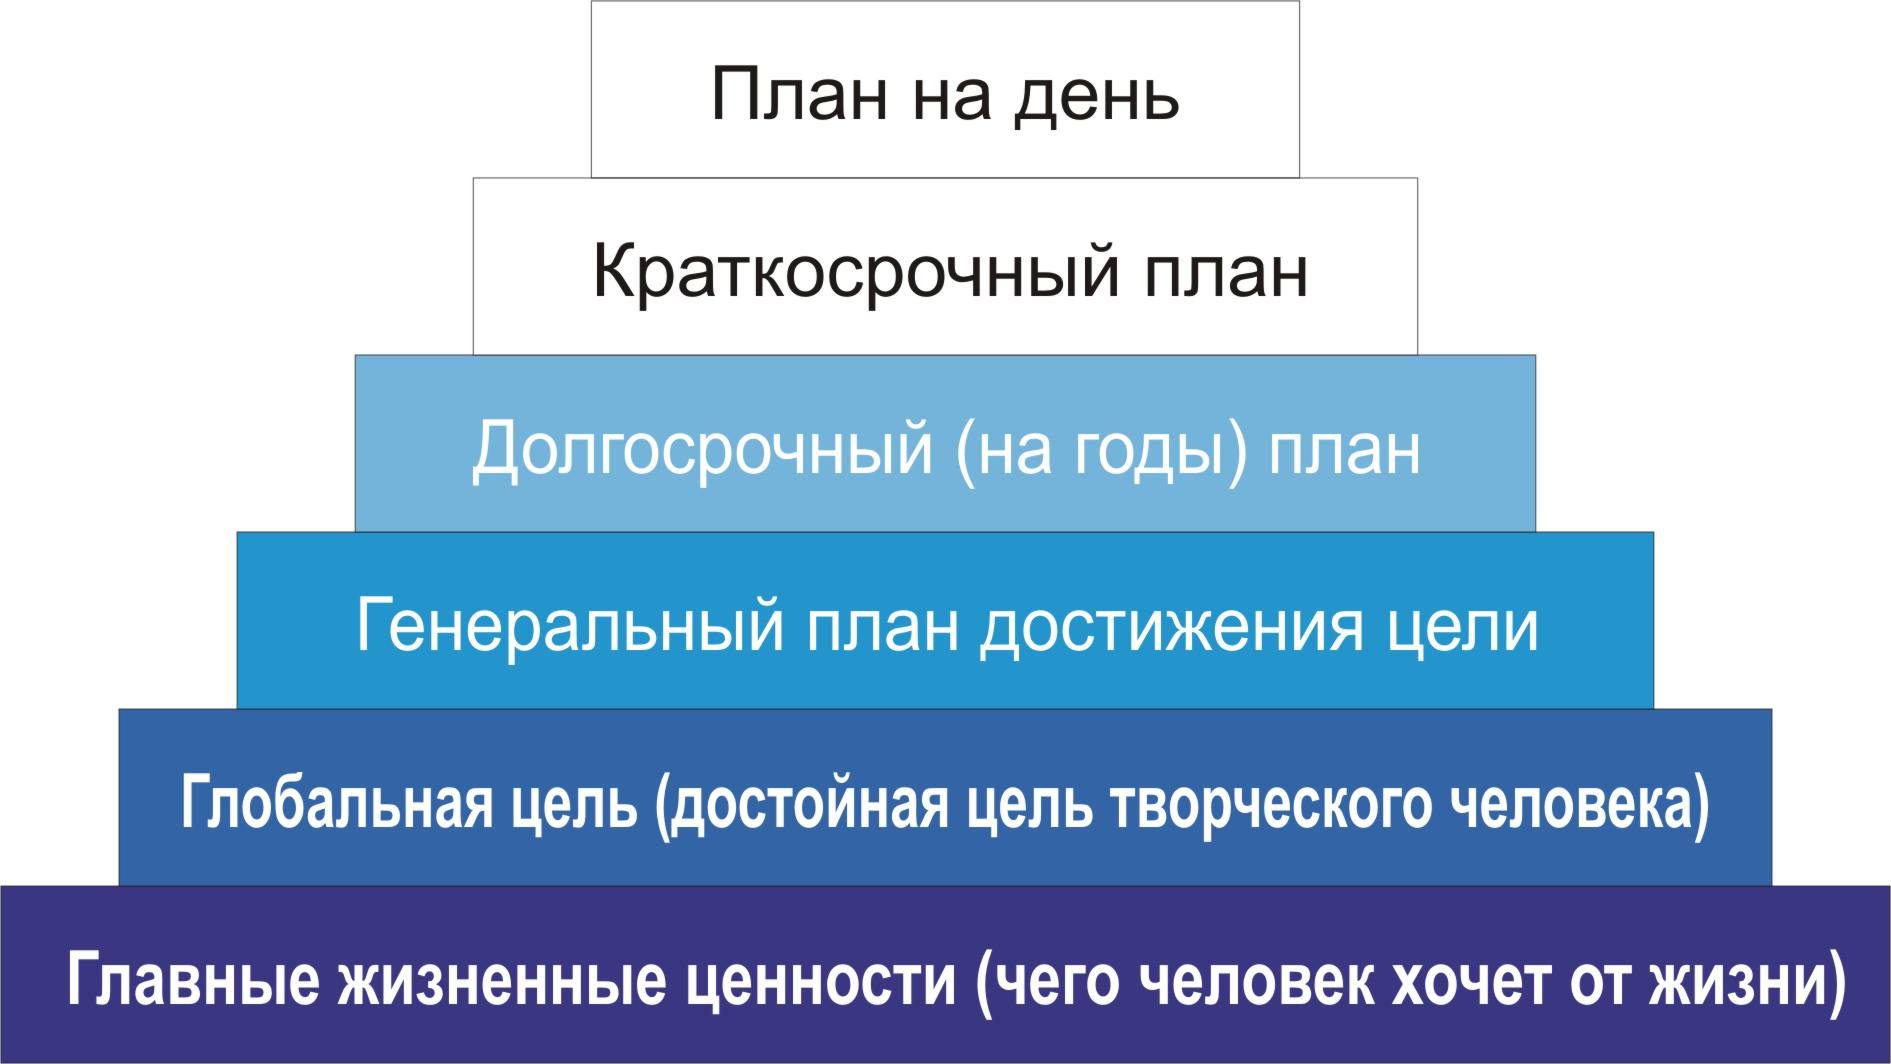
\includegraphics[scale=0.85]{images/franklin_piramida.jpg}
  \caption{ Пирамида Франклина }
  \label{fig:domain:franklin}
\end{figure}


Структура системы представляется как пирамида, где каждый элемент зависит от предыдущего это целостная система постановки и реализации целей. Ее главной особенностью является направленность на результат и планомерное движение от общего к частному. Весь жизненный распорядок, таким образом, подчинен достижению главных жизненных целей. Система Франклина имеет следующую структуру: жизненные ценности, глобальная цель, генеральный план, долгосрочный план, краткосрочный план, план на день. 


1. Жизненные ценности – это базовые глобальные ценности. Это ответ на вопросы: «Ради чего я живу?», «Что для меня является самым важным в жизни?». Очень важно искренне ответить для себя на эти вопросы и не ошибиться при их определении. Кто-то находит смысл жизни в признании, во власти, кто-то в семье, для кого-то важнее всего обеспеченная жизнь и деньги, для других самосовершенствование и альтруизм и т.д. Если речь идет об организации, то «жизненные цели» – это ее миссия, глобальное предназначение, смысл существования. Например, миссия компании «Отис» (производители лифтов и эскалаторов) звучит так: «Мы помогаем людям перемещаться в пространстве». Миссия нефтяной компании – «Мы обеспечиваем энергией». 

2. Глобальная цель ставится на основании заявленных жизненных ценностей. Это «большая» цель, максимально желаемая. Например, спортсмен-марафонец, определивший, что для него самое важное – слава и известность, признание мирового Олимпа, решает стать чемпионом мира. 

3. Генеральный план – это большой и общий план по достижению глобальной цели. Например, для того чтобы стать олимпийским чемпионом, нужно иметь хорошее здоровье и физическую форму, физкультурное образование, отличного тренера, получить звание мастера спорта, победить на соревнованиях области/города/страны/Европы. 

4. Долгосрочный план – это план на несколько лет, с указанием конкретных целей и сроков. Для спортсмена важно участвовать в соревнованиях Восточной Европы и победить там. Для этого ему нужно, чтобы показатели его скорости пробега были больше, чем у прошлого чемпиона. Необходимо сформулировать цель следующим образом: «К 2011 году я должен пробегать 42 км за 2 часа – так я завоюю титул чемпиона Восточной Европы и буду приглашен на чемпионат Мира». 

5. Краткосрочный план – план на срок от нескольких недель до нескольких месяцев. Исходя из долгосрочного плана, важно определить, что можно сделать в течение ближайших нескольких недель и месяцев для достижения цели. Так, для нашего спортсмена – это увеличить количество тренировок, повысить выносливость организма, опробовать новую систему подготовки. 

6. План на день. Задачи из плана на неделю разбиваются на более мелкие, например, задача увеличить выносливость выглядит как: пойти в спортзал, заниматься на беговом тренажере 3 часа, пробежать 5 км за 20 мин, замерить пульс, записать результаты в дневник.

\subsection{Матрица Эйзенхауэра}
Матрица Эйзенхауэра (матрица приоритетов) – один из самых известных инструментов для управления своим временем. Ее придумал Дуайт Эйзенхауэр, 34-й президент США.

Матрица Эйзенхауэра используется для планирования на небольшой срок (один или несколько дней). Это эффективный метод обработки тех списков дел, что человек планирует сделать за этот срок. Как правило, люди составляют столь длинные списки, что все дела из них априори невозможно переделать.

Представляет собой четыре квадранта, основанием которых служат две оси — это ось важности (по вертикали) и ось срочности (по горизонтали). В итоге получается, что каждый квадрант отличается своими качественными показателями. В каждый из квадрантов записываются все задачи и дела, благодаря чему образуется предельно ясная и объективная картина того, чем следует заняться в первую очередь, чем – во вторую, а чем вообще заниматься не стоит.

\label{page:domain:piramida_franklina}
\begin{figure}
\centering
  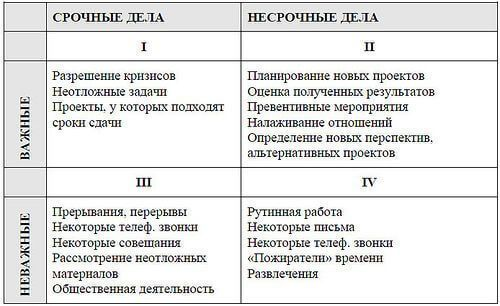
\includegraphics[scale=0.85]{images/eizinhower.jpg}  
  \caption{ Матрица Эйзенхауэра }
  \label{fig:domain:eizenhower}
\end{figure}

Организаторские способности Эйзенхауэра ценились всегда и везде. И совершенно заслуженно. Сейчас же матрицу Эйзенхауэра считают одним из самых эффективных средств для составления планов на короткий срок.



\subsubsection{Квадрант A: важные и срочные дела }


При идеальном планировании этот квадрант матрицы должен оставаться пустым, т.к. появление важных и срочных дел является показателем неорганизованности и допущения завала. Эта часть графика заполняется у многих людей из-за присущей им лени и неправильной расстановки приоритетов. Естественно, временами подобные дела могут появляться у каждого человека, но если это происходит ежедневно, то самое время обратить внимание на самодисциплину.

Итак, появления дел в квадранте A следует избегать. А для этого необходимо лишь вовремя выполнять пункты остальных квадрантов. Но если в первый квадрант что-то всё же и стоит вписывать, то это:

    Дела, невыполнение которых отрицательно сказывается на достижении поставленных целей
    Дела, невыполнение которых может стать причиной затруднений и неприятностей
    Дела, которые имеют отношение к здоровью

Важно также помнить о том, что существует такое понятие как «делегирование». Это означает, что при появлении в вашем квадранте A дел, которые можно кому-либо перепоручить, этой возможностью следует непременно воспользоваться для того чтобы как можно быстрее урегулировать другие важные и срочные дела.

\subsubsection{Квадрант B: важные, но не срочные дела }


Второй квадрант заслуживает наибольшего внимания, т.к. дела, находящиеся именно в нём, являются наиболее приоритетными и перспективными, и именно из них должны состоять повседневные задачи любого человека. Замечено, что люди, которые занимаются преимущественно делами этого квадранта, достигают в жизни наибольших успехов, продвигаются по службе, зарабатывают больше денег, имеют достаточно свободного времени и живут счастливой и насыщенной жизнью.

Обратите внимание также и на то, что отсутствие срочности позволяет подходить к решению любых задач более обдуманно и конструктивно, а это в свою очередь позволяет человеку раскрывать свой потенциал в полной мере, самостоятельно продумывать все нюансы своей деятельности и управлять временными рамками своих дел. Но здесь, помимо всего прочего, нужно помнить, что дела, находящиеся в квадранте B, если их не выполнять своевременно, могут с лёгкостью попасть в квадрант A, став ещё более важными и требующими скорейшего выполнения.

Опытные специалисты по организации времени рекомендуют включать в квадрант B все текущие дела, связанные с основной деятельностью, планирование и анализ работы, учебные и спортивные занятия, соблюдение оптимального графика и режима питания. Т.е. всё то, из чего состоит наша обычная повседневность.

\subsubsection{Квадрант C: срочные, но не важные дела }


Дела, которые находятся в этом квадранте, по большей части являются отвлекающими и нисколько не приближающими человека к намеченным результатам. Нередко они просто мешают сосредоточению на действительно важных задачах и снижают эффективность. Главное при работе с матрицей – не перепутать срочные дела из квадранта C со срочными делами из квадранта A. Иначе образуется неразбериха и то, что должно быть выполнено в первую очередь, остаётся на втором плане. Всегда помните о своих целях и учитесь отличать важное от второстепенного.

К делам квадранта C можно отнести, к примеру, навязанные кем-либо со стороны встречи или переговоры, празднования дней рождения не очень близких людей, внезапно возникшие хлопоты по дому, устранение не жизненно важных, но требующих внимания отвлекающих факторов (разбилась ваза, сломалась микроволновая печь, перегорела лампочка и т.п.), а также другие всевозможные дела, которые не продвигают вас вперёд, а только тормозят.

\subsubsection{Квадрант D: не срочные и не важные дела }


Задачи, относящиеся к последнему квадранту, не приносят совсем никакой пользы. Во многих случаях полезно не только заниматься ими в последнюю очередь, но и не заниматься ими вообще. Хотя знать о них непременно нужно, т.к. именно они являются «пожирателями времени».

Интересна и ещё одна особенность дел из данной группы: они являются очень привлекательными для многих людей – эти дела просты в выполнении и доставляют удовольствие, позволяют расслабиться и приятно провести время. Поэтому и противостоять соблазну ими позаниматься бывает довольно проблематично. Но делать это непременно нужно.

В квадрант D можно записать такие дела как разговоры по телефону с друзьями о чём-то несущественном, ненужная переписка или времяпрепровождение в соцсетях, просмотр сериалов и различных «отупляющих» телепередач, компьютерные игры и т.п. Конечно, отдыхать и как-то развлекать себя периодически должен каждый человек, но для этого существуют и более интересные и развивающие способы: чтение хороших книг, интеллектуальные игры, посещение спортзалов и бассейнов, поездки на природу и т.п. Если же полностью избавить себя от занятия делами из квадранта D не удаётся или не хочется, то нужно отложить их выполнение хотя бы до того момента, когда дела из квадрантов B и C будут выполнены, а время, которое будет уделяться делам квадранта D, должно быть сведено к минимуму.

\subsection{ Getting Things Done }

GTD, Getting Things Done — это система для самоорганизации, придуманная американским автором Дэвидом Алленом. С момента выпуска соответствующей книги в 2000 году миллионы неорганизованных людей наконец обрели счастье и душевное спокойствие. Ведь система, как заявляется, позволяет привети дела в порядок.

Основные принципы GTD очень просты. В основе лежат три привычки, к которым должен приучить себя каждый эффективный человек.
\begin{itemize}
  \item Записывать свои дела (Collect);
  \item Быстро решать, что делать дальше (Process);
  \item Делать то, что записал (Do).
\end{itemize}


\subsubsection{Collect }

Почему многие люди испытывают постоянный стресс и ничего не успевают? Потому, что они хранят все дела в голове. А мозг человека способен одновременно удерживать в памяти только 7 объектов. Если хранить в голове слишком много мусора, многие вещи просто забываются и вспоминаются только тогда, когда уже поздно. В итоге получаются все эти «Забыл», «Не успел», «Ай, сделаю завтра»…

Первым шагом на пути к светлой голове будет отложить на 10 минут все дела в сторону, взять листок бумаги и выписать все дела, вопросы, идеи и прочие вещи, которые не дают вам покоя. Тем самым мы освобождаем голову и переносим все свои дела на «внешний носитель».
Пример? Пожалуйста. Слушаю я радио, и вдруг слышу рекламу про наступающий праздник 8 марта. В голову сразу приходит мысль «Не мешало бы купить подарок маме». Не откладывая в долгий ящик, сразу записываю: «Купить подарок маме на восьмое марта».
Готово? Переходим к следующему пункту.

\subsubsection{Process }

На этом этапе нужно пройтись по всем записанным делам и для каждого из них задать себе один важный вопрос: какой следующий шаг?
Этот простой вопрос не так прост, как кажется. Например: вам нужно купить подарок маме и вы прилежно записали в блокнот «купить подарок маме на восьмое марта».
Что из этого получится? Скорее всего, вы будете долго искать себе отмазки, а подарок будет куплен в последний день. Ну и в результате накануне придется отстоять полдня в очередях, хотя на неделю раньше могли бы купить за пять минут.

Что в этом случае советует GTD.
GTD говорит вот что: сначала нужно выделить конкретный следующий шаг для покупки подарка. Конкретный шаг означает то, что ты оторвешься от стула и реально что-нибудь сделаешь. Например «Позвонить тете Ане и посоветоваться насчет подарка». Задача вдруг стала намного конкретнее, не правда ли? Теперь не нужно долго раздумывать: надо взять телефон и позвонить прямо сейчас.
Вот мы и пришли к третьему пункту.

\subsubsection{Do }

Если до этого было сделалано всё правильно, то на данном этапе есть простая и понятная задача: «Позвонить тете Ане».
Так получается потому, что конечным итогом применения системы GTD является «кристально чистый» список «следующих шагов» по всем задачам. В этом списке собраны конкретные и понятные дела, которые можно выполнять без раздумий. Все раздумия уже проведены на этапе «Что дальше»?..

Теперь, при наличии такого кристально чистого списка, можно спокойно и не отвлекаясь щелкать дела одно за одним, как семечки. Никаких лишних терзаний, никаких сомнений — сплошной концентрированный поток действия. 


\subsection{Обзор существующих аналогов } 
\label{sec:practice:analogs}

\subsubsection{Doit.im }
\label{sub:practice:analogs:doit}
Мультиплатформенный  сервис для учета времени, имеет клиенты на Windows, OSX, Android, IOs а также веб версию. Как и любой другой сервис учет времени позволяет создавать задачи, и группы этих задач.

Отличительные черты данного проекта:

\begin{itemize}
  \item возможность добавллять к задачам контекс (прим. Работа, Быт и.др);
  \item возможность добавлять задаче тэги, и группировать по ним;
  \item возмжность создания задачи задавая параметры (контекст, тэг, проект и т.д.) с помощью специальных символов. Например, если ввести: Забрать сына из школы \string^Today @Семья \#Быт !High \&Дети –  будет создана задача “Забрать сына из школы” с датой выполнения Сегодня, имеющая контекст Семья, помещенная в проект Быт, с высоким приоритетом и которой будет присвоен тэг Дети.
\end{itemize}

\begin{figure}[ht]
\centering
  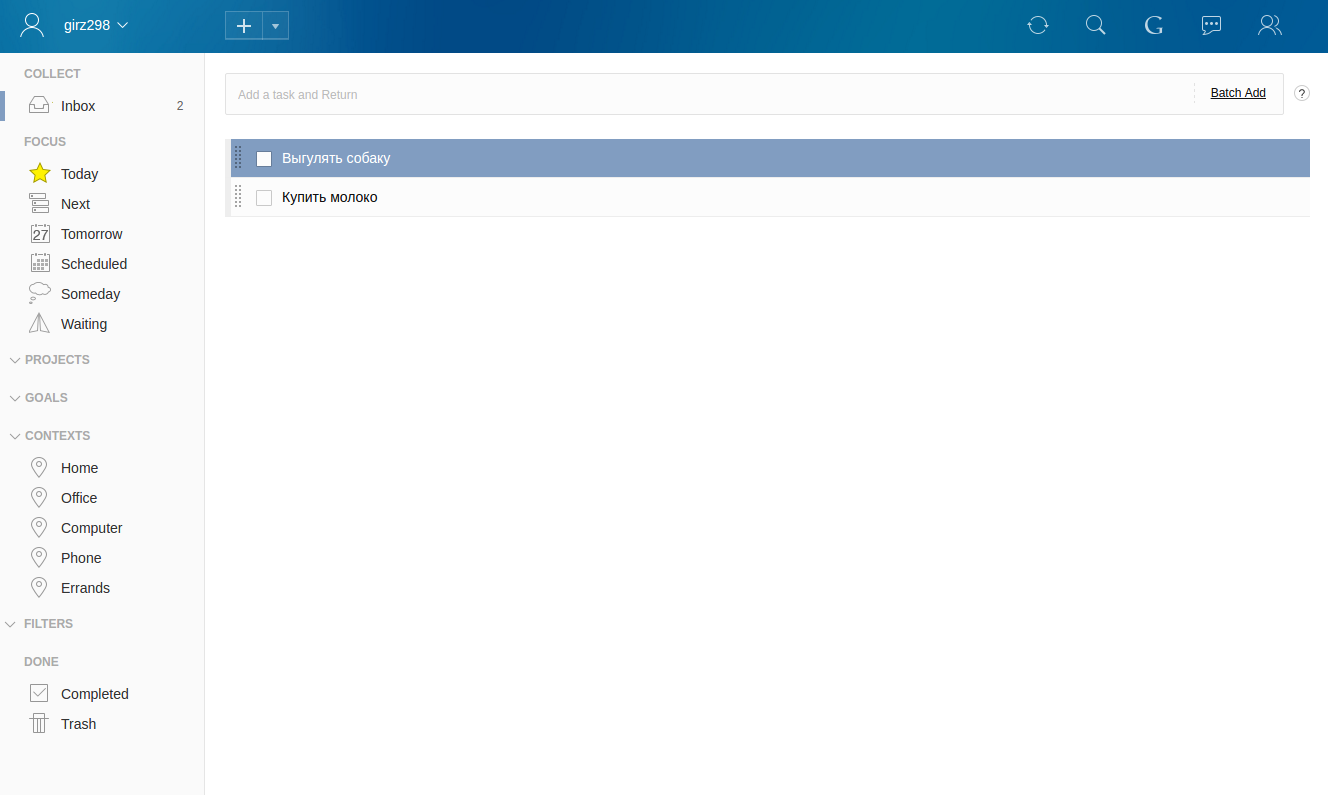
\includegraphics[scale=0.35]{images/doit.png}  
  \caption{ Основная страница веб-версии сервиса Doit.im }
  \label{fig:domain:doit.im}
\end{figure}

Doit.im — бесплатное приложение, однако ряд функций доступен только в PRO-версии. В любом случае бесплатно предоставляется 30-ти дневная бесплатная версия. Годовая подписка обойдется в \string$20. Еще один минус — отсутствие поддержки русского языка, кириллицу приложение распознает, но меню отображается только на английском. 

\subsubsection{Microsoft To-Do }
\label{sub:practice:analogs:microsoft_to_do}
Microsoft To-Do — это сервис для составления списка дел на день и распределения их по категориям. Функция «Интеллектуальные предложения» предложит оптимальный вариант распределения задач на основе прошлых записей. To-Do умеет импортировать задачи из Todoist и Wunderlist и синхронизироваться с приложениями из пакета Office. Доступно добавление заметок, напоминаний, повторов задач.

\label{page:domain:microsoft_to_do}
\begin{figure}[ht]
\centering
  
\includegraphics[scale=0.25]{images/microsoft_to_do.jpg}  
  \caption{ Мобильная и настольная версия Microsoft To-Do }
  \label{fig:domain:microsoft_to_do}
\end{figure}

\subsubsection{Remember the milk }
\label{sub:practice:analogs:remember_the_milk}

Этот сервис управления задачами считается одним из наиболее функциональных. Авторы Remember the Milk использовали принципы популярной техники управления задачами GTD, что и привело к появлению столь широкого набора функций. На первый взгляд количество параметров для задач в этом сервисе кажется слишком большим, и те пользователи, которым нужен просто список, наверняка не будут играться с заполнением всех этих полей. Для задачи в Remember the Milk можно указать срок выполнения, настроить повтор, задать ее продолжительность, добавить теги, место, ссылку, текстовые заметки, приоритет. Список мест формируется в специальном разделе и помогает напомнить, например, купить продукты в супермаркете, выполнить рабочие задачи в офисе и не забыть о домашней рутине, когда человек оказался дома. 

\begin{figure}[ht]
\centering
  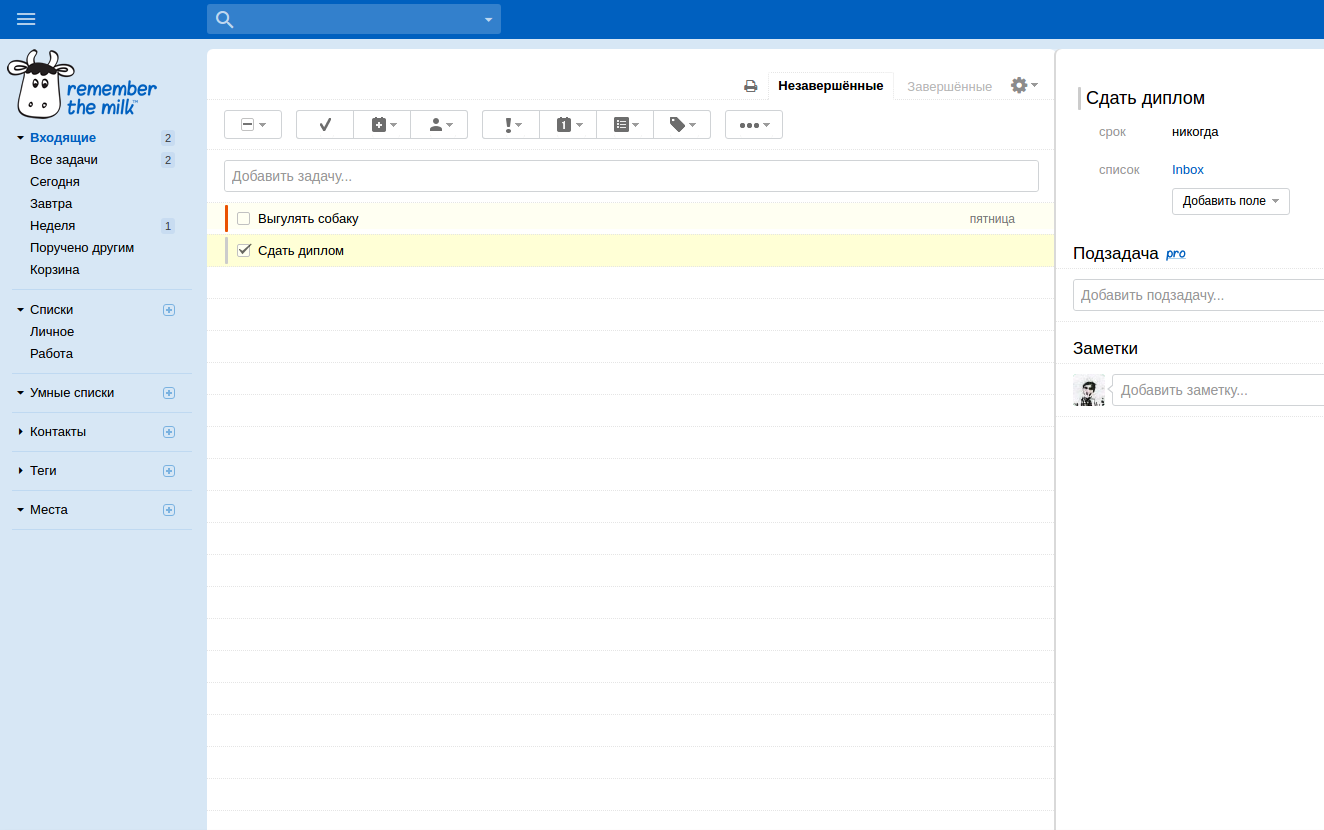
\includegraphics[scale=0.35]{images/remember_the_milk.png}  
  \caption{  Основная страница веб-версии сервиса Remember The Milk }
  \label{fig:domain:remember_the_milk}
\end{figure}

Отличительные черты данного проекта:

\begin{itemize}
  \item "умные" списки. Группируют задачи по спискам, классифицируя их по ключевым словам, заданным в описании этого списка;
  \item работа с геолокацией;
  \item список контактов;
  \item возможность давать задачи пользователям из списка контактов.
\end{itemize}

В отличии от сервиса Doit.im в него добавлена полная поддержа русского языка, а также неплохой вводный курс на русском языке. Однако бесплатная версия ограничивается малой долей функционала. За полноценную PRO-версию без ограничений функционала авторы просят \string$40 в год.

\subsubsection{Todoist }
\label{sub:practice:analogs:todoist}

Кроссплатформенный проект с многомилионной аудиторией. Имеет интеграцию с многими сервисами, облачную синхронизацию, интуитивно понятный интерфейс и полную русскую локализацию. Для работы нужно создать новый проект(группу задач), затем добавить в него задачи, указав их описание и планируемые сроки выполнения.  Приоретизация задач основана на матрице Эйзенхауэра. 

Отличительные черты данного проекта:

\begin{itemize}
  \item есть возможность создание команды(группы пользователей) и командного выполнения задач;
  \item приоритизация задач основана на матрице Эйзенхауэра;
  \item отличная кроссплатформенная поддержка от Apple Watch до Symbian устройств.
\end{itemize}


\begin{figure}[ht]
\centering
  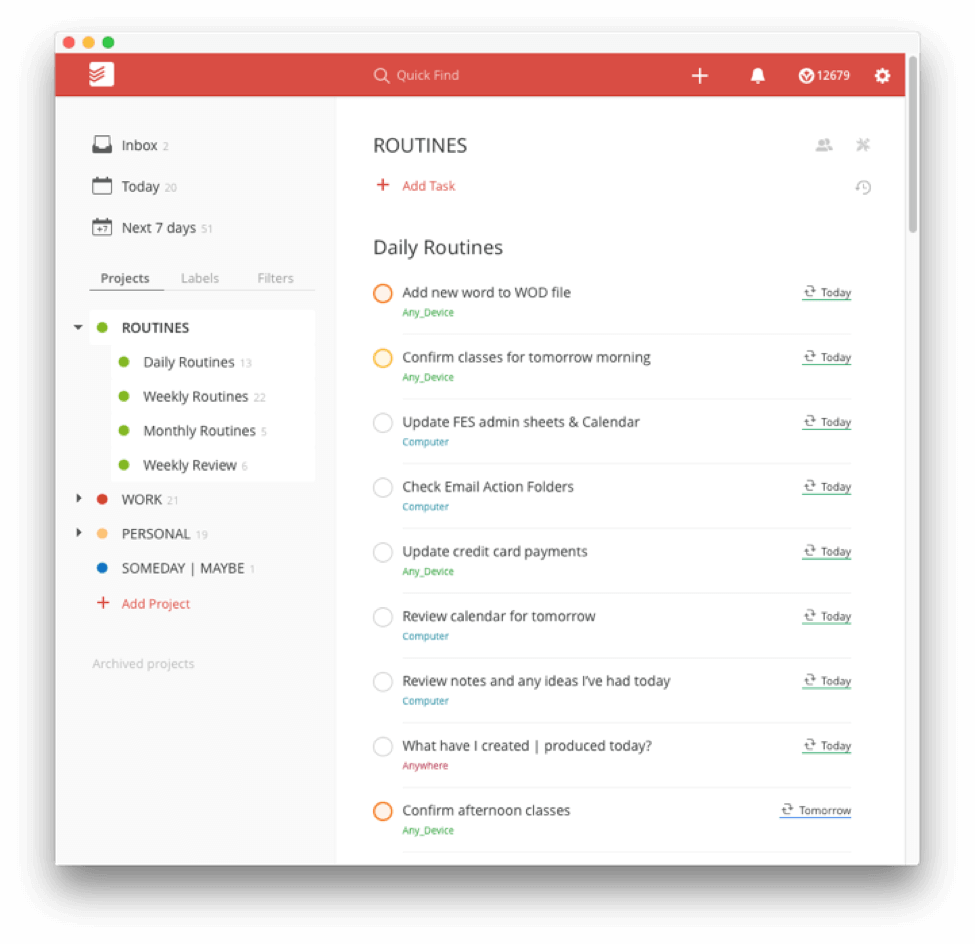
\includegraphics[scale=0.42]{images/todoist.png}  
  \caption{  Основная страница веб-версии сервиса Todoist }
  \label{fig:domain:todist}
\end{figure}

Также как и в аналогичных сервсах у этого есть PRO-версия стоимостью \string$29 в год. Пользователи с PRO-версией могут добавлять комментарии к своим задачам, просматривать завершённые задачи, отправлять задачи по электронной почте, получать напоминания на почту или через SMS, экспортировать задачи в календарь Google, Outlook или iCal, использовать поиск и просматривать статистику своей продуктивности по дням и проектам.